\section{Fly-Through Core}
\label{sec:FlyThrough}

\begin{figure*}
    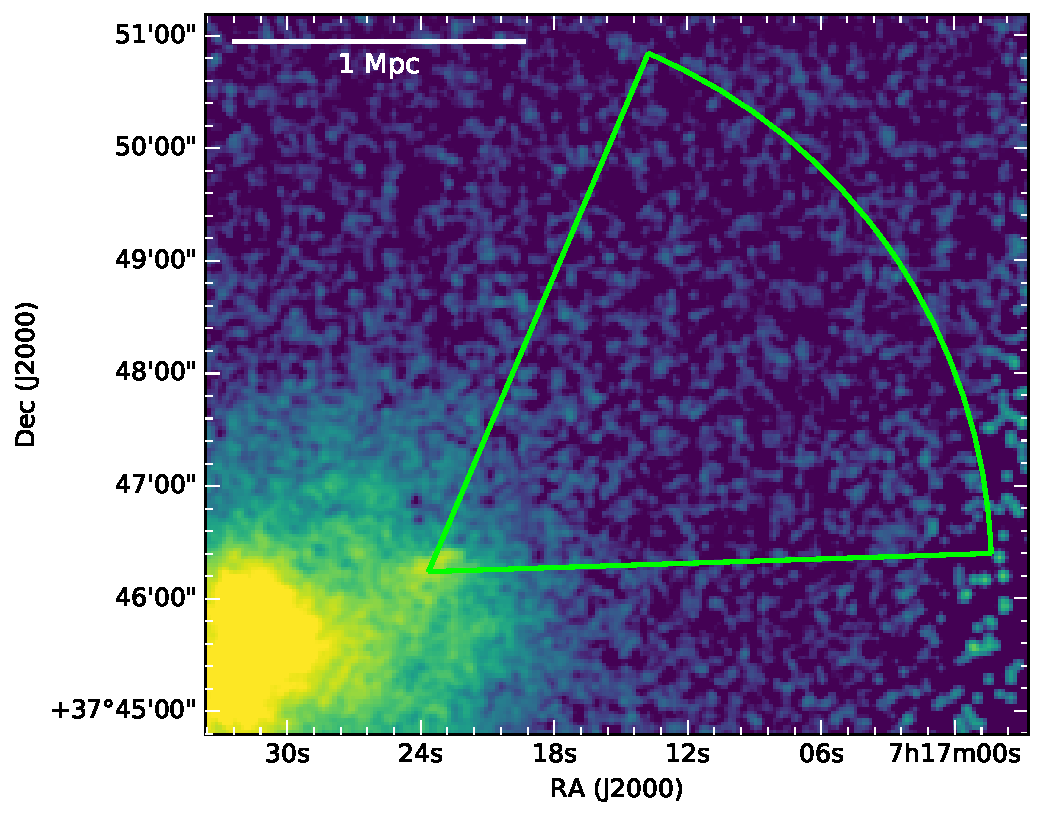
\includegraphics[width=\columnwidth]{plots/circ-panda.pdf}
    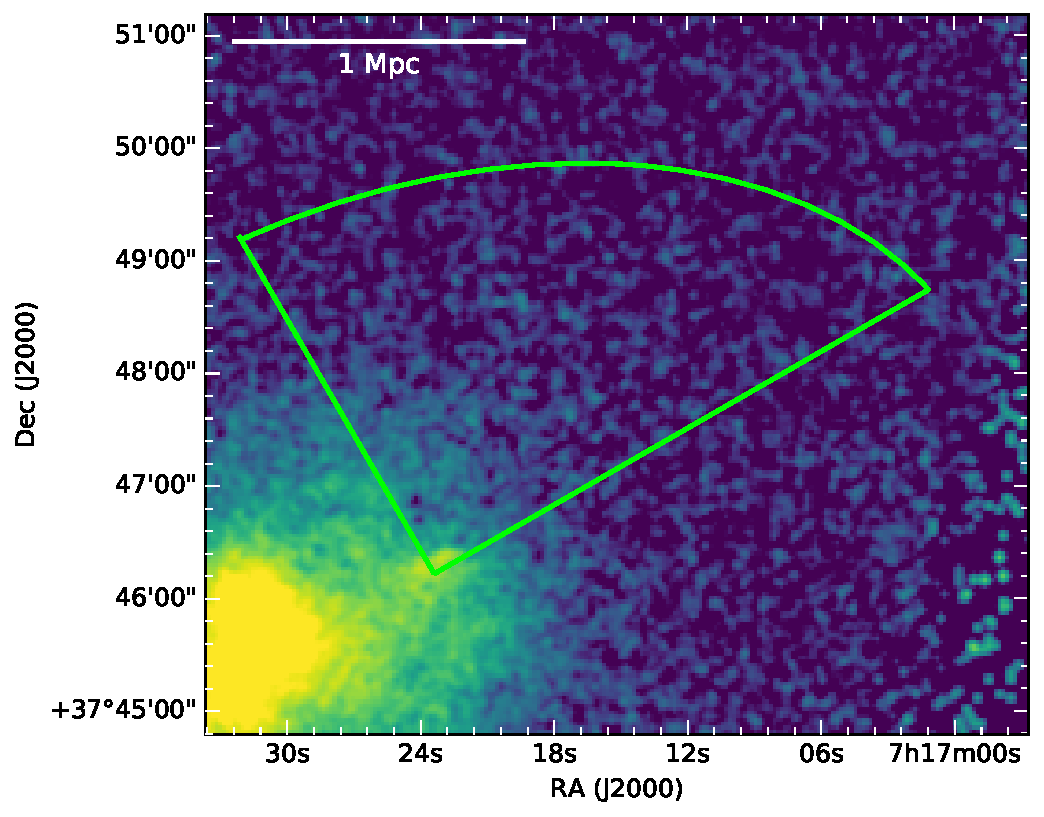
\includegraphics[width=\columnwidth]{plots/ell-panda.pdf}
    \includegraphics[width=0.33\textwidth]{plots/{macsj0717-core-circ-beta}.pdf}
    \includegraphics[width=0.33\textwidth]{plots/{macsj0717-core-ell-beta}.pdf}
    \includegraphics[width=0.33\textwidth]{plots/{macsj0717-core-ell-bknpow}.pdf}
    \caption{\emph{Top:} Sectors used to model the surface brightness profile in front of the core. \emph{Bottom:} Surface brightness profiles and best-fitting models. The instrumental background is shown in blue, with the uncertainty ranges on the background shown in dashed blue lines. For the elliptical sector, the surface brightness is plotted against the major axis of the ellipse. The best-fitting parameters of the broken power-law model are listed in Table~\ref{tab:bknpow}. \label{fig:sectors}}
\end{figure*}

\begin{table*}
  \caption{Best-fitting parameters of the broken power-law model fitted to the surface brightness of the core. Uncertainties are quoted at the $1\sigma$ level. The region from which the surface brightness profile was extracted, as well as the profile and best-fitting model, are shown in Figure~\ref{fig:sectors}.\label{tab:bknpow}}
  \begin{center}
    \begin{threeparttable}
      \begin{tabular}{c c c c c c}
              $\alpha_1$\tnote{a} & $\alpha_2$\tnote{b} & Normalization & $r_{\rm break}$ & $n_1/n_2$\tnote{c} &  Sky background \\
                               &        &     photons cm$^{-2}$ s$^{-1}$ arcmin$^{-2}$       & arcmin   & &    photons cm$^{-2}$ s$^{-1}$ arcmin$^{-2}$ \\
              \hline
              $0.62 \pm 0.44$ & $1.09 \pm 0.15$ & $(1.82 \pm 1.11)  \times 10^{-4}$ & $0.30\pm 0.05$ & $1.61\pm 0.40$ & $(1.24 \pm 0.17) \times 10^{-6} $ \\
      \end{tabular}
      \begin{tablenotes}
              \item[a] Power-law index at $r < r_{\rm break}$.
              \item[b] Power-law index at $r > r_{\rm break}$.
              \item[c] Density jump across the discontinuity.
      \end{tablenotes}
    \end{threeparttable}
  \end{center}
\end{table*}

Approximately 670 kpc NW of the cluster center, there is a bright X-ray core with a tail extending $\sim 200$~kpc towards SE, roughly in the direction of the large-scale filament discussed in Section~\ref{sec:Filament}. This morphology suggests that this core, seen `flying' through the ICM of MACS~J0717.5+3745 and ram-pressured stripped by the cluster's dense ICM, traveled NW along the SE filament and is seen after it traversed the brightest ICM regions. In essence, the core is a later stage of the group currently seen within the filament. 

The core is embedded (at least in projection) in the ICM of MACS~J0717.5+3745. To determine the core's physical properties, we  modeled the contamination from the ICM by extracting spectra N and S of the core. These spectra were modeled with a thermal component with a metallicity of 0.2 solar. We assumed the spectral properties were the same in the N and S regions. The spectra of the core were modeled as the sum of emission from the contaminating ICM and from the core itself. The spectra of the core and of the regions N and S of it were modeled in parallel. The best-fitting results are summarized in Table~\ref{tab:spectra}. The temperature of the core, $6.82_{-1.36}^{+1.88}$~keV, is consistent with the temperatures N and S of the core, in regions that are approximately at the same distance from the cluster center as the core. We also compared the core temperature with the temperatures ahead of (NW) and behind (SE) the core. The temperature decreases from $10.89_{-1.27}^{+2.05}$~keV behind the core, to $5.06_{-0.98}^{+1.61}$~keV ahead of the core. From these temperature measurements, we therefore find no evidence of a core colder than its surroundings, nor of a temperature discontinuity (either a shock or a cold front) ahead of the core. 

A cold front and a shock front would be expected ahead of the core, similarly to the features seen in the Bullet Cluster \citep{Markevitch2002} and in front of the group NGC 4839 infalling into the Coma Cluster \citep{Neumann2001} ***other citation needed here for the cold front***. We searched for possible evidence of a cold/shock front by modeling the surface brightness profile of the group. The sectors from which the surface brightness profiles were extracted are shown in the top panels of Figure~\ref{fig:sectors}. We chose two sectors: a circular sector with an opening aligned with the apparent direction of motion of the core, and an elliptical sector with an opening and ellipticity aligned with a possible edge observed by eye in the surface brightness map. The models fitted to these surface brightness profiles are shown in the bottom panels of Figure~\ref{fig:sectors}. The surface brightness profile extracted from the circular sector is well-fitted by a $\beta$-model. In this profile, there is a suggestion of an edge near $\sim 0.3$~arcmin, but a surface brightness model based on a broken power-law density model did not significantly improve the fit. In the surface brightness profile extracted from the elliptical sector, this possible edge becomes clearer. A $\beta$-model fit to this profile provides a good fit at high radii, but not at distances below $\lesssim 0.5$~arcmin. As seen in the bottom-right panel of Figure~\ref{fig:sectors}, a broken power-law density model follows the data closer. The best-fitting broken power-law density model fitted to the surface brightness profile in the elliptical sector has a density jump of $1.88\pm 0.35$ at $\approx 0.27$~arcmin from the center of the sector. The best-fitting parameters for the broken power-law model are summarized in Table~\ref{tab:bknpow}.

The density discontinuity is at the very edge of the core. Therefore, we speculate that the discontinuity is associated with a cold front rather than with a shock front. The failure to find a temperature discontinuity associated with the density jump is likely due to a combination of poor count statistics and hot gas projected onto the core. The latter would also dampen the observed density jump, in which case our measurement of the jump amplitude is only a lower limit.  


